\documentclass{article}
\usepackage{amsmath}
\usepackage{tikz}
\usetikzlibrary{matrix}

\begin{document}

\begin{figure}[h]
    \centering
    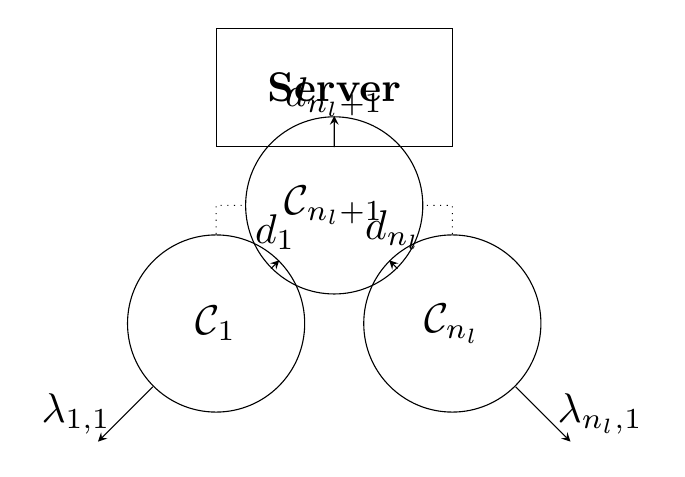
\begin{tikzpicture}[scale=1.5, transform shape]
        % Define styles for nodes
        \tikzstyle{server} = [draw, rectangle, minimum width=2cm, minimum height=1cm,text centered, font=\bfseries]
        \tikzstyle{cache} = [draw, circle, minimum width=1.5cm, minimum height=1cm, text centered]
        \tikzstyle{arrow} = [->, >=stealth]

        % Draw the server node
        \node[server] (server) at (0, 3) {Server};

        % Draw the cache nodes
        \node[cache] (cache1) at (-1, 1) {$\mathcal{C}_1$};
        \node[cache] (cacheml) at (1, 1) {$\mathcal{C}_{n_l}$};
        \node[cache] (cachemlplusone) at (0, 2) {$\mathcal{C}_{n_l+1}$};

        % Draw the arrows between nodes
        \draw[arrow] (server) -- node[above] {$d_{n_l+1}$} (cachemlplusone);
        \draw[arrow] (cachemlplusone) -- node[above] {$d_1$} (cache1);
        \draw[arrow] (cachemlplusone) -- node[above] {$d_{n_l}$} (cacheml);

        % Draw the arrows from the leaves to the caches
        \draw[arrow] (cache1) -- node[left] {$\lambda_{1,1}$} ++(-1, -1);
        \draw[arrow] (cacheml) -- node[right] {$\lambda_{n_l,1}$} ++(1, -1);

        % Draw the dotted lines from the cache to the server
        \draw[dotted] (cache1) -- ++(0, 1) -- (cachemlplusone);
        \draw[dotted] (cacheml) -- ++(0, 1) -- (cachemlplusone);
    \end{tikzpicture}
    \caption{Two level cache hierarchy tree consisting of $n_l$ leaves. The random variable $d_i$ encodes the random delay for cache $i$ to download the content from its parent. The server is assumed to contain all objects. The request rate of object $i$ at leaf $j$ is denoted $\lambda_{i,j}$.}
    \label{fig:cache_hierarchy}
\end{figure}

\end{document}